\documentclass[a4paper]{jpconf}
\bibliographystyle{iopart-num}
\usepackage{amsmath}
%\usepackage{citesort}
\usepackage{subfigure}
\usepackage{graphicx}
\graphicspath{{fig/}}
\usepackage{ifpdf}
\ifpdf\usepackage{epstopdf}\fi
\usepackage[export]{adjustbox}
\usepackage[numbers]{natbib}
%----------------------------------------------------- 
%\usepackage{soul,ulem,color,xspace,bm}
% Suggest to remove
%\newcommand{\asrm}[1]{{\color{magenta}\sout{#1}}}
% Suggest to insert
%\newcommand{\as}[1]{\color{cyan}#1\xspace\color{black}}
% Suggest to replace
%\newcommand{\asrp}[2]{\asrm{#1} \as{#2}}
% Comment
%\newcommand{\ascm}[1]{{\color{green}\;AS: #1}}
%------------------------------------------------------

\def\apj{ApJ}
\def\mnras{MNRAS}
\def\nat{Nat}
\def\prd{Phys. Rev. D}
\def\araa{ARA\&A}                % "Ann. Rev. Astron. Astrophys."
\def\aap{A\&A}                   % "Astron. Astrophys."
\def\aaps{A\&AS}                 % "Astron. Astrophys. Suppl. Ser."
\def\aj{AJ}                      % "Astron. J."
\def\apjs{ApJS}                  % "Astrophys. J. Suppl. Ser."
\def\pasp{PASP}                  % "Publ. Astron. Soc. Pac."
\def\apjl{ApJ}                   % letter at ApJ
\def\pasj{PASJ}
\def\apss{Astroph. Space Sci.}
\def\aplett{Astroph. Lett}
\def\ssr{Space Sci. Rev.}
\def\aapr{Astron. Astroph. Reviews}
\def\physrep{Phys. Reports}
\def\memsai{Mem. Societa Astronom. Italiana}
\def\jgr{JGR}
\def\jcap{Journal of Cosmology and Astroparticle Physics}
\def\nar{New Astronomy Reviews}

\usepackage{xspace}
\usepackage[dvipsnames]{xcolor}
\usepackage[normalem]{ulem}
% Suggest to remove
\newcommand{\asrm}[1]{{\color{OrangeRed}\sout{#1}}}
% Suggest to insert
\newcommand{\as}[1]{\color{RoyalBlue}#1\xspace\color{black}}
% Suggest to replace
\newcommand{\asrp}[2]{\asrm{#1} \as{#2}}
% Comment
\newcommand{\ascm}[1]{{\color{ForestGreen}#1}}

\begin{document}
	\title{Kinetic modeling of MHD parameters of mildly-relativistic shocks}
	
	\author{V I Romansky$^{1}$, A M Bykov$^{1,2}$ and S M Osipov$^{1}$}
	
	\address{$^1$ Ioffe Institute, 26 Politekhnicheskaya st., St. Petersburg 194021, Russia}
	\address{$^2$ Peter the Great St. Petersburg Polytechnic University, 29 Politekhnicheskaya st., St. Petersburg 195251, Russia}
	
	\ead{romanskyvadim@gmail.com}
	
	\begin{abstract}
    Mildly-relativistic outflows with shocks of  velocities  $0.1 - 0.7 c$ were deduced from multiwavelength observations of powerful fast transient sources. These outflows are associated with  merging relativistic objects, relativistic supernovae and fast blue optical transients. Relativistic  magneto-hydrodynamic (RMHD) models of this objects rely on the equation of state of the fluid which is a collisionless plasma with a contribution of non-thermal components. In this paper we present kinetic simulations of mildly-relativistic shocks with - Particle-in-Cell and Monte-Carlo techniques to derive the adiabatic index of plasma in shock downstream  directly from particle distributions which can be implemented into RMHD models. 
	\end{abstract}
	

\section{Introduction} 
Recent multiwavelength observations of fast energetic transient sources associated with some classes of supernova and neutron star mergers revealed a presence there of mildly-relativistic outflows with shock waves of velocities faster than 0.1c \citep{2016ApJ...819...35A,2019ApJ...872...18M,2020ApJ...895...49H,2021ApJ...912L...9N,2019LRR....23....1M,2021ARA&A..59..155M,2021ApJ...911..104K,2022ApJ...927L..17H}. 
Analysis of 42 day-timescale evolving transients detected with Zwicky Transient Facility (ZTF) \citep{ZTF_stat_Ho21} suggested that most of these are likely associated with core-collapse supernovae (SNe). The authors  distinguished a few sub-types of the typical events as   (i) subluminous SNe of Type Ib or IIb; (ii) luminous Type Ibn or hybrid IIn/Ibn SNe; and (iii) short-duration radio-loud luminous events which prototype is nearby AT2018cow event. While the subluminous SNe events of Type IIb are the most numerous the AT2018cow like events rate is less than 0.1\% of the local core-collapse SNe rate \citep{ZTF_stat_Ho21}. The multiwavelength data on fast SNe related transients can be generally understood assuming an action of a powerful central engine  in the collapsing stars which can launch a relativistic jet-type outflow. Relativistic hydrodynamical  simulations  performed in \citep{2012ApJ...750...68L,2021NewAR..9201614C} illustrated that depending on the time duration of the central engine power activity either GRB type jet source (for a long enough activity time) or, for a shorter power injection time, somewhat broader outflow and radio bright relativistic SN can be produced by a collapsing star. The different energy injection regimes by the central engine result in different energy versus the ejecta speed distributions. The powerful jet breaking through the stellar envelope can form  a mildly-relativistic expanding cocoon containing the energy $\sim$ 10$^{51}$ ergs (see e.g. \citep{2019ApJ...871L..25P}).    
The the cocoon interacting with the circumstellar winds may emit the synchrotron self-absorbed radio emission observed in fast optical transients \citep{2022MNRAS.tmp..970G}. The physical models of particle acceleration in fast transients based on particle in cell simulations of mildly-relativistic shocks in barionic plasma produced by the central engine activity in the fast transients were discussed in \cite{BRO22_Univ}. The mildly relativistic shocks are also determining the transition from the early highly-relativistic to the later time semi-relativistic likely barion-dominated outflows in the gamma-ray burst afterglows (see e.g. \citep{Piran04,Meszaros06,GRBafterglow_hydro12}) where the models can be used to model the non-thermal radiation. Moreover, mildly relativistic shocks in stellar mass transient sources can be considered as efficient accelerators of cosmic rays well above PeV regime (see \citep{2018SSRv..214...41B} and the references therein). The future  Large Synoptic Survey Telescope will detect a large amount of fast transients providing a good possibilities to of the follow up multiwavelength studies. Therefore there is clear need in detailed modeling of different appearances of the semi-relativistic outflows in the transient sources. While to model the global structure of the flows the RMHD simulations are widely used the collisionless shocks need the microscopic kinetic type of simulations since the collisionless shocks are producing non-thermal components which may influence the equation of state and the macroscopic parameters like the adiabatic indexes of the semi-relativistic plasma. Therefore we present below the results of a simulations of macroscopic plasma parameters which can be used in the global RMHD simulations.      
 

\section{Particle-in-Cell simulation}
In this work we use particle-in-cell code Smilei \cite{Smilei18} for modeling collisionless shocks. Simulation domain is two-dimensional with reflective wall on the left boundary along the x axis and the plasma flowing in through the right boundary. Boundary conditions along the y axis are periodic.

The simulation parameters are : the initial flow Lorentz factor $\Gamma$ is in interval $1.05-1.5$ for different setups, the flow magnetization $\sigma = \frac{B^2}{4\pi\Gamma (n_0 m_p + n_0 m_e) c^2} = 0.0002$, where B is magnetic field, $m_p$ and $m_e$ are proton and electron masses, $c$ is speed of light. Upstream concentration $n_0$ is equal to $1$, but all quantities can be easily scaled to different value. The temperature $T = 0.02$ in units of the electron rest energy and the electron mass is increased up to $m_e = \frac{m_p}{100}$. We used setups with different velocities of plasma flow $v_u = \beta_u c$ and inclination angles of magnetic field: $\theta$ is angle between the magnetic field and the flow velocity and $\phi$ is angle of field rotation in perpendicular plane, $\phi=0$ corresponds to the magnetic field lying in the simulation plane. Setups and they parameters are listed in table \ref{setups}. The spatial grid step is $dx = 0.2 c/{\omega_p}$ and the time step $dt = 0.1/{\omega_p}$, where $\omega_p = \sqrt{\frac{4\pi q^2 n_0}{m_e}}$ is the plasma frequency, $\displaystyle q$ is the
absolute value of the electron charge. The size of the simulation box along the $x$ axis is $L_x = 40000\frac{c}{\omega_p}$ and in the transverse direction $L_y = 100\frac{c}{\omega_p}$. These scales correspond to $200000$ and $500$ grid points in $x$ and $y$ directions, respectively. 

We obtain MHD parameters of the shock from the simulation. The position of the shock front is well defined as shown in figure \ref{density_noturb} so we can evaluate the shock velocity in the downstream frame $v^d_{sh}$  and $\beta^d_{sh} = {v^d}_{sh}/c$. The shock velocity in the upstream frame is defined as $\beta_sh = (\beta_u + \beta^d_{sh})/(1 + \beta_u \cdot\beta^d_{sh})$.
	\begin{figure}[h!]
		\centering
		\begin{minipage}{0.49\textwidth}
			\centering
			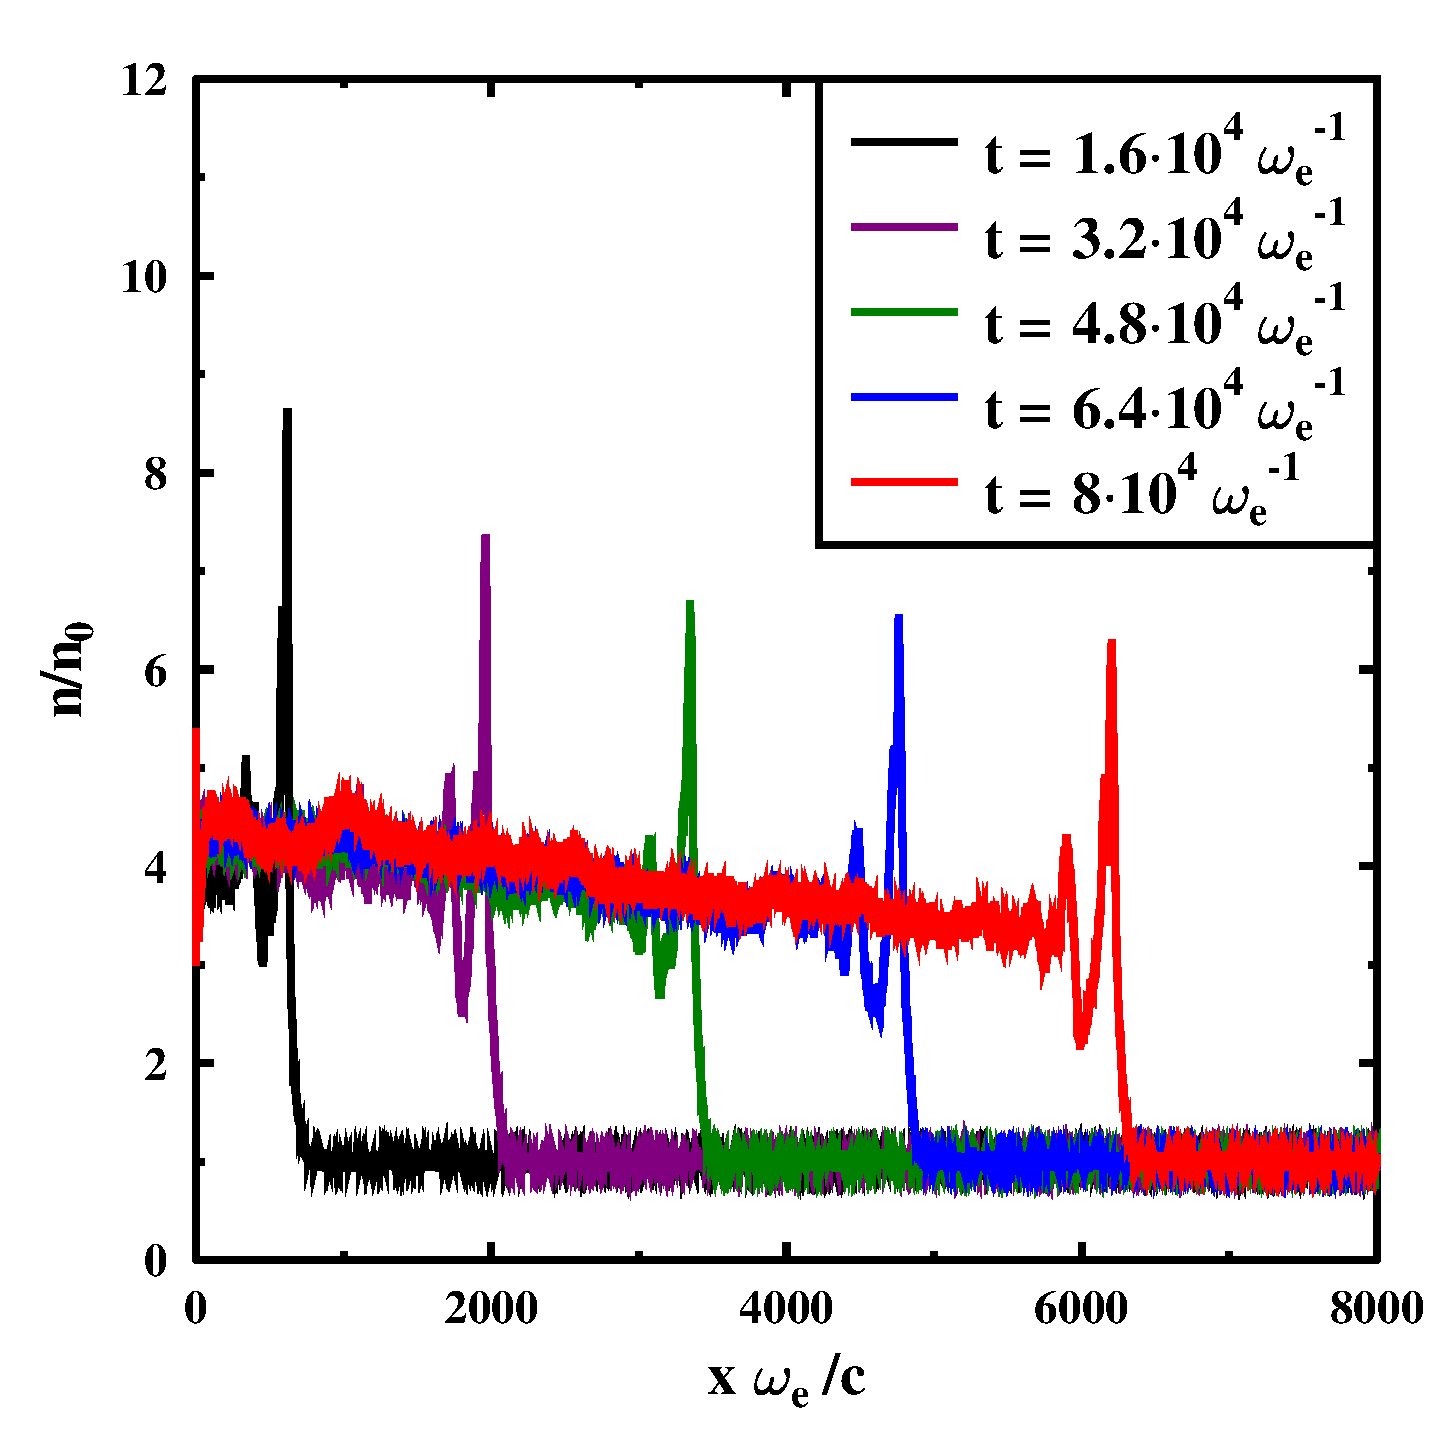
\includegraphics[width=0.98\textwidth]{concentrations.eps} 
			\caption{Time evolution of concentration normalized to the far upstream~concentration, setup B30.}
			\label{density_noturb}
		\end{minipage}\hfill
		\begin{minipage}{0.49\textwidth}
			\centering
			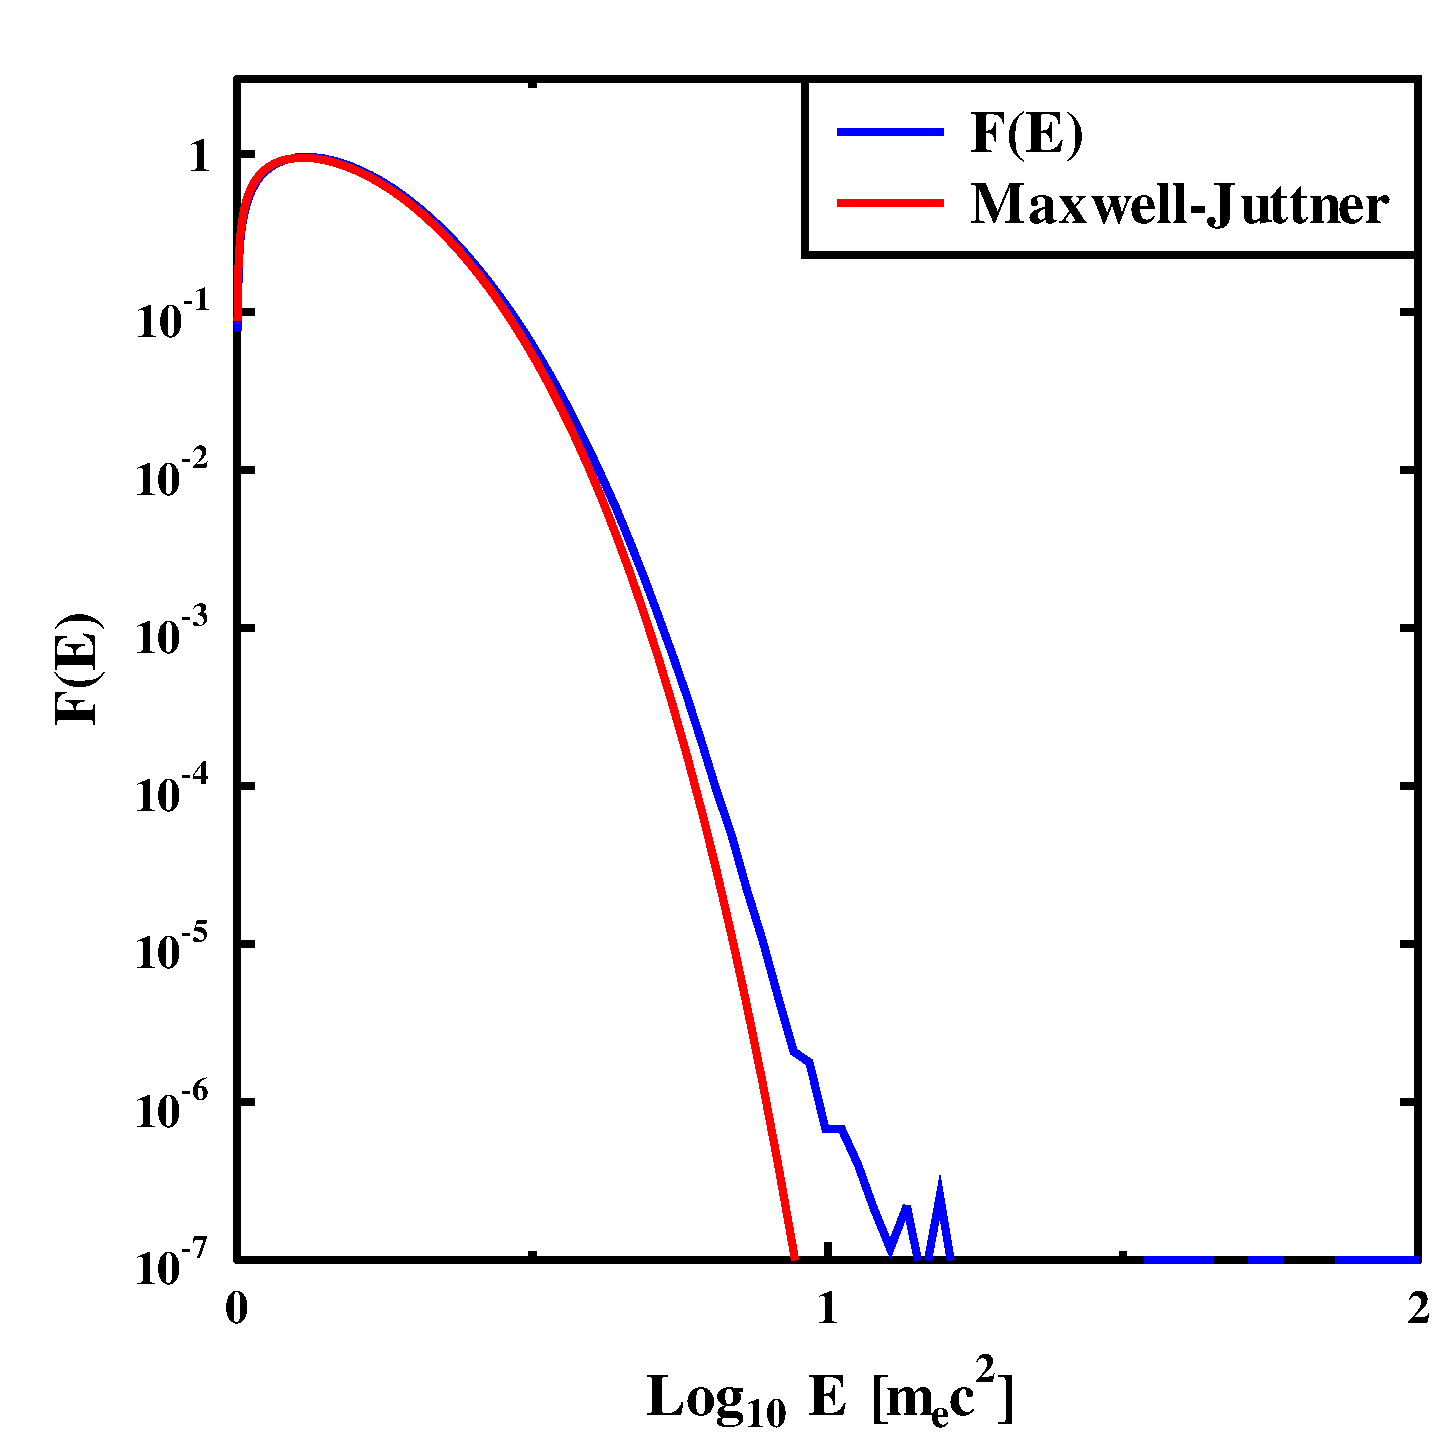
\includegraphics[width=0.98\textwidth]{electrons2.eps} 
			\caption{Fit of the electron distribution in the shock downstream with Maxwell-Juttner distribution, setup B30.}
			\label{density_turb}
		\end{minipage}
	\end{figure}
We can find temperature of every particle species behind the shock, minimizing the 
functional $\displaystyle f(T) = \int_{m c^{2}}^{5 m c^{2}} (F(E) - F_{mj}(E,T))^{2}dE$, where $\displaystyle F(E)$ is simulated distribution function and $\displaystyle F_{mj}(E,T)$ is Maxwell-Juttner distribution function. Also we can derive adiabatic index for every species of particles using definition $\gamma_i = 1 + P/E_k$ where $P$ is the pressure and  $E_k$ is the kinetic energy of particles in the plasma rest frame. $P = \int F(E) v_x(E,\theta) p_x(E,\theta) 2 \pi sin(\theta) d\theta dE$ and $E_k = \int F(E) (E - m c^2) 2 \pi sin(\theta) d\theta dE$. Also we define $\hat\gamma$ - the adiabatic index, evaluated with same formulae but using the Maxwell-Juttner particle distribution with the corresponding temperature.
	\begin{table}[h!]
	\label{setups}
	\caption{Parameters of different setups. }
	\begin{center}
		\begin{tabular}{|c | c| c| c| c| c| c| c| c| c| c| c|}
			\hline
			Setup & $\theta$ & $\phi$ & ${\beta}_u$ &  ${\beta^d}_{sh}$ & ${\beta}_{sh}$ & ${\gamma}_p$ & ${\gamma}_e$ & $T_p\ 10^{10}K$ & $T_e \ 10^{10}K$ & $\hat{\gamma}_p(T_p)$ & $\hat{\gamma}_e(T_e)$\\
			\hline
			A30 & 30 & 90 & 0.5 &  0.13 & 0.59 & 1.620 & 1.389 &75.5 & 19.0 & 1.617 & 1.389\\
			A80 & 80 & 90 & 0.5 & 0.16 & 0.61 & 1.601 & 1.396 &54.7 & 16.3 & 1.629 & 1.397\\	
			B30  & 30 & 90 & 0.3  & 0.088 & 0.38 & 1.647 & 1.499 & 14.5 & 4.0 & 1.656 & 1.502\\
			B50  & 50 & 90 & 0.3  & 0.098 & 0.39 & 1.648 & 1.468 & 11.0 & 5.9 & 1.658 & 1.469\\
			C30  & 30 & 0 & 0.3  & 0.088 & 0.38 & 1.647 & 1.502 & 14.4 & 3.9 & 1.656 & 1.504\\
			D30 & 30 & 90 & 0.1 &  0.035 & 0.135 & 1.665 & 1.574 &1.9 & 1.3 & 1.665 & 1.589\\
			D80 & 80 & 90 & 0.1 & 0.052 & 0.151 & 1.664 & 1.580 &2.6 & 1.5 & 1.665 & 1.579\\
			\hline
		\end{tabular}
	\end{center}
    \end{table}
    
    
One can see from the table that adiabatic index obtained from PIC simulation is smaller than from simple hydrodynamic theory. It should be taken into account in MHD simulations. This difference increases when particle acceleration is more efficient (case of quasi-parallel shock). Also, PIC simulation can not simulate long non-thermal tales of distributions because of it's high computational cost, and other methods, such as hybrid and Monte-Carlo simulation are needed for more precise modeling of MHD parameters.

\section{Monte Carlo simulation}	
Due to the limited computing power, PIC modeling can be performed only in a small area of the volume of real astrophysical objects. To describe astrophysical objects on their real scales, it is necessary to involve other numerical models. One of such models is Monte Carlo calculations, which, unlike PIC calculations, require the introduction of phenomenological laws, such as the mean free path of particles, the growth rates of plasma instabilities.


We develop a nonlinear numerical stationary plane-parallel relativistic Monte Carlo model of particle acceleration by longitudinal collisionless shocks \cite{BRO22_Univ}. Particle acceleration occurs by the first-order Fermi mechanism. The particles are scattered by magnetic fluctuations and repeatedly cross the shock front. In our model, on the basis of an iterative scheme, the conservation laws of energy and momentum fluxes near the shock are fulfilled. The model takes into account the modification of the upstream by the pressure of accelerated particles, the amplification of magnetic fluctuations due to plasma instabilities caused by the anisotropy of the accelerated particle distribution function in the upstream, the dissipation of turbulent modes, and the turbulent cascade. Particle propagation is organized on the basis of pitch-angle scattering. The particles are divided into acceleration and background. An accelerated particle is considered if it has crossed the front of the shock at least once from the downstream to the upstream.


The Table~\ref{MC_calculations} shows the results of Monte Carlo calculations for different shock velocities $u_{sh}$ ($\beta_{sh}=u_{sh}/c$). ${\gamma}_{th}$, ${\gamma}_{cr}$, ${\gamma}_{tot}$ are the adiabatic indices of the background plasma, the accelerated particle distribution and the total in the downstream, respectively. $T_{th}$ is the temperature of background protons in the downstream. Other model parameters except $u_{sh}$ are the same in all calculations. The free escape boundary of particles is at the coordinate $x_{FEB}=-5\cdot 10^{14}$ cm, the shock front corresponds to the coordinate x = 0. The number density of the background plasma $n_{0}=5\cdot 10^{5}$ cm$^{-3}$ in the far unperturbed upstream. The rms turbulent magnetic field $B_{st}\left(x_{FEB}\right)$ is equal to the constant magnetic field $B_{0}=3\cdot 10^{-3}$ G in the far unperturbed upstream. $B\left(x\right)=\sqrt{B_{st}^{2}\left(x\right)+B_{0}^{2}}$.


	\begin{table}[h!]
	\label{MC_calculations}
	\caption{Results of Monte Carlo calculations. }
	\begin{center}
		\begin{tabular}{|c | c| c| c| c| c| }
			\hline
			Setup  & ${\beta}_{sh}$ & ${\gamma}_{th}$ & ${\gamma}_{cr}$ & ${\gamma}_{tot}$ & $T_{th}\ 10^{10}K$ \\
			\hline
			MC1  & 0.1 & 1.66 & 1.43 & 1.49 & 0.59 \\
			MC2  & 0.3 & 1.66 & 1.42 & 1.49 & 7.11 \\
			MC3  & 0.5 & 1.64 & 1.41 & 1.49 & 26.5 \\
			MC4  & 0.7 & 1.61 & 1.40 & 1.48 & 82.4 \\
				
			\hline
		\end{tabular}
	\end{center}
    \end{table}


The Figure~\ref{u_B_eff_MC1} shows the profiles of the background plasma flow velocity and the magnetic field. The turbulent part of the magnetic field is amplified due to plasma instabilities and adiabatically. $r_{g0}=m_{p}cu_{sh}/eB_{0}$, where $e$ is elementary charge.
    
    
\begin{figure}[h!]
\begin{center}
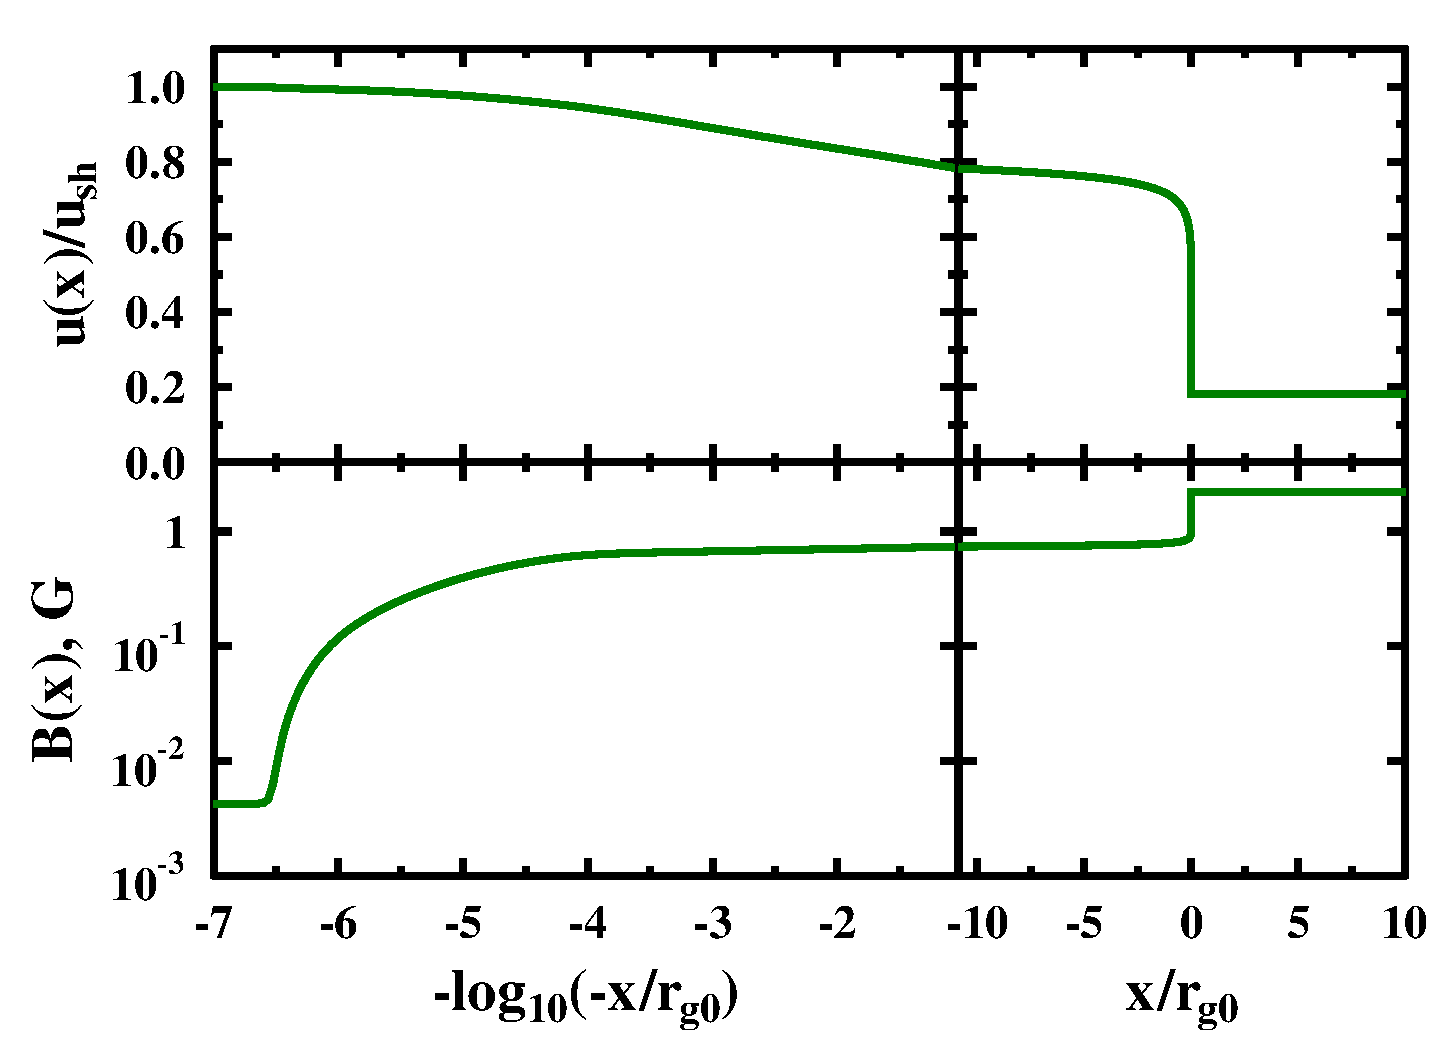
\includegraphics[scale=0.5]{u_B_eff_MC1.eps}
\end{center}
\caption{Background plasma velocity profile (upper panel) and magnetic field profile (bottom
panel) for the Monte Carlo calculation MC1.}
\label{u_B_eff_MC1}
\end{figure}


The scales achievable in PIC modeling are of the order of several $r_{g0}$. That is, PIC modeling can describe a small area near the shock compared to Monte Carlo modeling (see Figure~\ref{u_B_eff_MC1}). Since the maximum energies of accelerated particles strongly depend on the size of the system, in Monte Carlo calculations, the maximum energies of particles are many orders of magnitude higher than in PIC calculations. The temperature of the background plasma in the downstream in Monte Carlo simulation is also affected by the amplification of modes by plasma instabilities associated with the anisotropy of the distribution of  high-energy accelerated particles and the energy dissipation of these modes at the upstream scales.
	
\section{Conclusions}
Hydrodynamic and RMHD models are constructed to interpret the light-curves and spectra of fast transients (e.g. \citep{1999ApJ...510..379M,2012ApJ...750...68L,2019LRR....23....1M,2020ApJ...903...66L,2021ApJS..256....8U,2022MNRAS.tmp..970G,2022arXiv220108432E} and the reference therein).
The parameters obtained in kinetic modeling of MHD shocks with non-thermal components can be used in the hydrodynamic modeling of  global structures of fast mildly-relativistic outflows.	
	
	
\ack
	Some results of the work were obtained using computational resources of Peter the Great Saint-Petersburg Polytechnic University Supercomputing Center (http://scc.spbstu.ru)
	
%\section*{References}

%\providecommand{\newblock}{}

%\begin{thebibliography}{10}
%\expandafter\ifx\csname url\endcsname\relax
%  \def\url#1{{\tt #1}}\fi
%\expandafter\ifx\csname urlprefix\endcsname\relax\def\urlprefix{URL }\fi
%\providecommand{\eprint}[2][]{\url{#2}}
% Bibliography created with iopart-num v2.0
% /biblio/bibtex/contrib/iopart-num


% \bibliographystyle{apalike}
\bibliographystyle{iopart-num}

\bibliography{FBOT_bibl1}
%	
	
\end{document}